%\pstart
%[140 r\textsuperscript{o}] Il faut remarquer neantmoins quoyque l'experience refuteroit l'hypothese, que le mouuement des liqueurs en tous \edtext{sens ne meriteroit pas d'estre rejetté pour cela, estant seulement reconnu trop foible pour estre cause d'une union si}{\lemma{sens}\Afootnote{ \textit{ (1) }\ ne seroit pas r  \textit{ (2) }\ ne [...] bulle. \textit{ L}}} \edtext{forte, comme la nostre.}{\lemma{forte,}\Afootnote{comme la nostre. \textit{ erg.} \textit{ L}}}\pend
\pstart
[140 r\textsuperscript{o}] Il faut remarquer neantmoins quoyque l'experience refuteroit l'hypothese, que le mouuement des liqueurs en tous \edtext{sens ne meriteroit pas}{\lemma{sens,}\Afootnote{ \textit{ (1) }\ ne seroit pas r \textit{ (2) }\ ne meriteroit pas \textit{L}\ }} d'estre rejetté pour cela, estant seulement reconnu trop  foible pour estre cause d'une union si \edtext{forte, comme la nostre.}{\lemma{comme}\Afootnote{la nostre. \textit{ erg.} \textit{ L}}}  Peut estre même qu'on découuriroit ce mouuement par ses effects, en poursuivant cette sorte d'experiences avec  des corps plus \edtext{legers,}{\lemma{legers,}\Afootnote{\textbar\ propres pour cet effect;  \textit{ gestr.} \textbar\ et \textit{ L}}}  et je crois que \edtext{Mons. Rohault}{\lemma{Mons. Rohault}\Bfootnote{\textsc{J. Rohault}, \cite{00087}\textit{Traíté de physique}, Teil 1, Paris 1671, Kapitel 12, insbesondere §§ XXV\textendash XXIX.\protect\rule[0cm]{10cm}{0cm}}} nous a donné  déja quelque chose de cette nature. Enfin la même \edtext{demonstration  de nostre experience feroit son effect}{\lemma{}\Afootnote{ \textit{ (1) }\  fait son effect de la \textit{ (2) }\ de nostre experience feroit son effect contre \textit{erg.} \textit{L}}} contre toute autre  sorte de mouuements d'une matiere plus  subtile que \edtext{l'air, qu'on pourroit employer}{\lemma{l'air,}\Afootnote{ \textit{ (1) }\  dont on se pourroit servir \textit{ (2) }\  qu'on pourroit employer \textit{L}}} pour pousser ou presser les corps joincts l'un  contre l'autre. Car quoyque je croy qu'on ne  pourra pas se \edtext{passer icy}{\lemma{icy}\Afootnote{\textit{ erg.} \textit{ L}}} aisement d'une telle matiere \edtext{au moins selon la facon ordinaire de parler}{\lemma{au}\Afootnote{[...] parler \textit{ erg.} \textit{ L}}}, je croy pourtant aussi qu'il \edtext{suffiroit supposer son existence, sans se mettre}{\lemma{suffiroit}\Afootnote{ \textit{ (1) }\   la supposer simp \textit{ (2) }\  supposer son existence \textit{L}}} en peine de son mouuement.
\pend
                        \pstart
Pour approfondir d'avantage l'union  des corps purgez d'air, dont nous cherchons  la raison il faut examiner les phenomenes  jusqu'à la moindre circumstance; et surtout  cette Bulle d'air laquelle arrivant à une  certaine hauteur fait tomber l'eau purgée jusqu'  au dessous de cette hauteur. Soit dans la fig. 1  le \edtext{Recipient \textit{EE} le vase \textit{F}}{\lemma{Recipient}\Afootnote{ \textit{ (1) }\   epuisé \textit{ (2) }\   \textit{EE} le vase \textit{F} dans lequel l'eau purg\'{e}e \textit{L}}}  dans lequel l'eau purgée arrive jusqu'in A en sorte
  \edtext{que la bouche}{\lemma{que} \Afootnote{\textit{ (1) }\  le \textit{ (2) }\   la bouche \textit{L}}} du matras renversé \textit{CD}\textendash\textit{A} plein  d'eau purgée, trempe dans l'eau du vase \textit{F}.  Cela fait, et le Recipient estant épuisé à  force de pomper, le \edtext{matras ou la phiole}{\lemma{ou}\Afootnote{ la phiole \textit{ erg.} \textit{ L}}} ne se vuide pas, ce qu'il  feroit si l'eau n'estoit pas purgée.\pend
%Zeitz auskommentiert  \begin{center}                    
%                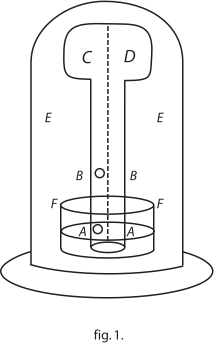
\includegraphics[width=0.4\textwidth]{images/37_3_140r4}\\\textit{[Fig. 4]}
%                        %\caption{Bildbeschreibung}
%                        \end{center}
%                        %@ @ @ Dies ist eine Abstandszeile - fuer den Fall, dass mehrere figures hintereinander kommen, ohne dass dazwischen laengerer Text steht. Dies kann zu einer Fahlermeldung fuehren. @ @ @ \\

  \pstart Il arrive cependant quelque fois, qu'une petite bulle d'air estant  parüe au fond de l'eau \textit{A} dans la superficie  interieure du Matras, grossissant peu à peu, et  montant jusqu'à une certaine hauteur \textit{B} s' étend  de là subitement vers en haut, et occupant tout  l'espace \textit{CD}\textendash\textit{B} fait descendre l'eau de la phiole,  et se mettre au dessous de \textit{B}. Et il semble que \textit{B} est plus haut ou plus bas à raison de la \edtext{hauteur de l'eau et de la}{\lemma{hauteur}\Afootnote{de l'eau et de la \textit{ erg.} \textit{ L}}} quantité  d'air dans la \edtext{bulle.
Car l'eau detachée une fois du haut \textit{CD} descend par son propre poids et il n'en reste au bas de la phiole,  que ce que le ressort du peu d'air qui est demeuré  dans le recipient peut soûtenir, quoyque l'air de la bulle,  qui occupe à present l'espace \textit{CD}\textendash\textit{B} soit plus dilaté que celuy  du Recipient. Mais si l'air de la phiole seroit moins dilaté,}{\lemma{bulle.}\Afootnote{\textit{ (1) } , l'eau descendant jusqu'à ce  que l'espace \textit{CD}\textendash\textit{B} devienne assez grand pour  faire l'air de la bulle \textbar\ dans la phiole  \textit{erg.} \textbar\  prendre le même degré de  dilatation que l'air du Recipient a déja. \textit{ (2) } . Car [...] poids \textit{ (a) } jusque \textit{ (b) } et il n'en reste \textit{ (aa) } dans \textit{ (bb) } au [...] present \textit{ (aaa) } la phiole \textit{ (bbb) } l'espace [...] Recipient. \textit{ L}}}
[140 v\textsuperscript{o}] que celuy du Recipient, il agiroit par son ressort\protect\index{Sachverzeichnis}{ressort}, et feroit l'eau descendre plus bas que sa pesanteur\protect\index{Sachverzeichnis}{pesanteur} ne demande, et par consequent le point \textit{B} ne \edtext{determineroit}{\lemma{ne}\Afootnote{ \textit{ (1) }\ seroit \textit{ (2) }\ determineroit \textit{ L}}} pas precisement la hauteur de la liqueur que l'air \edtext{du Recipient}{\lemma{}\Afootnote{du Recipient \textit{ erg.} \textit{ L}}} hors de la phiole peut so\^{u}tenir. \edtext{Ce qui peut arriver en effect:}{\lemma{}\Afootnote{Ce [...] effect: \textit{ erg.} \textit{ L}}} Car quoyqu'il ne peut jamais estre plus haut, il pourra quelque fois estre plus bas. Mais il sera regulierement le m\^{e}me. \edlabel{Mercurestart}\textso{Si l'on feroit l'experience avec du }\textso{Mercure}\protect\index{Sachverzeichnis}{mercure}\textso{ }\edtext{}{\lemma{\textso{Si} [...] \textso{Mercure:}}\xxref{Mercurestart}{Mercureend}\Afootnote{\textit{Markierung am Rand}}}\edtext{\textso{purg\'{e}}}{\lemma{}\Afootnote{\textso{purg\'{e}} \textit{ erg.} \textit{ L}}}\textso{ dans l'air libre, il est \`{a} croire que laissant entrer une bulle d'air, }\edtext{\textso{le point }\textit{\textso{B}}\textso{ seroit un peu au dessous de la hauteur ordinaire du Mercure} \edlabel{Mercureend}}{\lemma{\textso{d'air,}}\Afootnote{ \textit{ (1) }\ \textit{\textso{B}}\textso{ tombe} \textit{ (2) }\ \textso{le }[...] \textso{Mercure} \textit{ L}}} selon le calcul de \textso{Mons. }\edtext{\edlabel{mario140v}\textso{Mariotte}\edlabel{mario140v2}}{\lemma{\textso{Mons.}}\Afootnote{ \textit{ (1) }\ \textso{l'Abb\'{e}} \textit{ (2) }\ \textso{Mariotte} \textit{ L}}}\edtext{,}{\lemma{\textso{Mariotte,}}\xxref{mario140v}{mario140v2}\Bfootnote{Die Notiz beruht sehr wahrscheinlich auf einer persönlichen Begegnung. Eine Rechnung dieser Art findet sich 1676 in Mariottes \cite{00245}\textit{Discours de la nature de l'air}. Vgl. \textsc{E. Mariotte}, \textit{Oeuvres}, Bd. 1, Leiden 1718, S. 154f.}} mais cela ne sera pas considerable \edtext{icy}{\lemma{}\Afootnote{icy \textit{ erg.} \textit{ L}}}, \edtext{\`{a} moins que la}{\lemma{icy,}\Afootnote{ \textit{ (1) }\ si la \textit{ (2) }\ \`{a} moins que la \textit{ L}}} quantit\'{e} d'air qu'on a fait entrer \edtext{soit grande}{\lemma{entrer}\Afootnote{ \textit{ (1) }\ n'est pas grande \textit{ (2) }\ soit grande \textit{ L}}}.
\pend 
\pstart Il me semble tres difficile de rendre raison des phenomenes de la bulle, par le mouuement \edtext{en tous sens}{\lemma{}\Afootnote{en tous sens \textit{ erg.} \textit{ L}}} du fluide\protect\index{Sachverzeichnis}{fluide} ambient: car pourquoy ce mouuement \edtext{dans tout le Recipient}{\lemma{}\Afootnote{dans tout le Recipient \textit{ erg.} \textit{ L}}} est il surmont\'{e} par l'interposition d'une petite bulle d'air, dans la petite capacit\'{e} de laquelle la matiere subtile\protect\index{Sachverzeichnis}{mati\`{e}re!subtile} ne peut pas former tant de vagues, ny donner tant de coups, que dans le Recipient entier? Puisque \`{a} ce qu'on a respondu \`{a} l'objection des pores, la suspension depend de la quantit\'{e} des vagues ou coups. Si la suspension dependoit du mouuement de l'air\protect\index{Sachverzeichnis}{mouvement!de l'air} plustost, que d'une matiere\protect\index{Sachverzeichnis}{mati\`{e}re!subtile} plus subtile que l'air, on pourroit dire que l'air de la petite bulle, estant press\'{e}, \'{e}gale l'air dilat\'{e} du Recipient: mais ayant renonc\'{e} \edtext{\`{a} l'air}{\lemma{}\Afootnote{\`{a} l'air \textit{ erg.} \textit{ L}}} on ne peut pas s'en servir; outre qu'il falloit alors que la bulle d'air n\'{e}e dans la liqueur ou qu'on a fait entrer soit d'une telle consistence, que la liqueur estant tomb\'{e}e, et la bulle remplissant l'espace vuide\protect\index{Sachverzeichnis}{espace vide} dans le tuyau ou dans la phiole; soit justement \edtext{d'un degr\'{e} de pression}{\lemma{justement}\Afootnote{ \textit{ (1) }\ de la consistence \textit{ (2) }\ d'un degr\'{e} de pression \textit{ L}}} \'{e}gal \`{a} celuy de l'air de dehors. Ce qu'on peut refuter, \`{a} ce que je croy, par l'experience, si par hazard cette opinion trouueroit un defenseur, en se servant \edtext{dans l'air libre du Mercure purg\'{e}}{\lemma{servant}\Afootnote{ \textit{ (1) }\ du Mercure\protect\index{Sachverzeichnis}{mercure|textit} purg\'{e} suspendu dans un tuyau dans l'air li \textit{ (2) }\ dans [...] purg\'{e} \textit{ L}}}. Car ayant fait entrer une petite bulle \edtext{dans le tuyau}{\lemma{dans}\Afootnote{ le tuyau \textit{ erg.} \textit{ L}}}, et le mercure\protect\index{Sachverzeichnis}{mercure} estant tomb\'{e}, il faudroit que l'air qui occupe l'espace\protect\index{Sachverzeichnis}{espace vide} vuide au haut du tuyau soit d'une densit\'{e} \'{e}galle \`{a} celle de l'air ambient, ce qui est impossible, la bulle ayant est\'{e} petite quand elle \'{e}galoit cette densit\'{e}, c'est \`{a} dire quand on la faisoit entrer; et \`{a} present estant necessairement dilat\'{e}e pour occuper un si grand espace.